\textbf{Пример пары заданий одного типа, на основе которых создан следующий шаблон. } 

\begin{figure}[h]
		\centering
		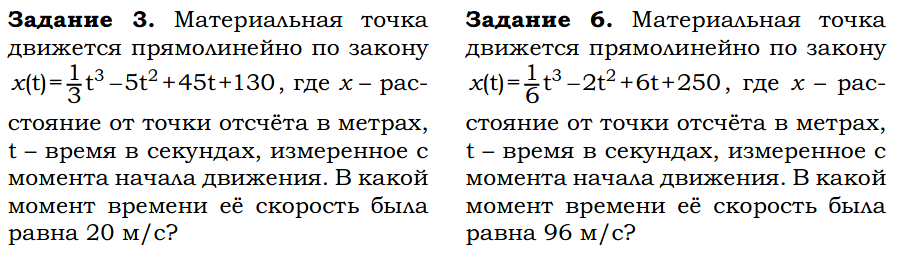
\includegraphics[width=1\linewidth]{VM/Пример.png}
\label{ris:image}
\end{figure}

Первая часть шаблона выглядит следующим образом:

\lstinputlisting{paragrafs/Zadachi/1}

Здесь объявляются переменные таким образом, чтобы генерируемые значения,  максимально соотносились с исходной задачей.

В этой части также используются специальные встроенные функции, такие как:
\\ \texttt{sluchch(a, b)} – функция случайным образом возвращает число из диапазона от «a» до «b». Если функции добавить третье число \texttt{sluchch(a, b, с)}, то она будет возвращать случайно число уже с шагом «с».
\\ \texttt{Math.abs(a)} – функция возвращает модуль числа «a».
\\ \texttt{function plusmin(member)} – функция принимает аргумент, содержащий в себе пример, наподобие: «1*a+-b». И возвращает его упрощённый вариант: «a-b».

Вторая часть выглядит следующим образом:

\lstinputlisting{paragrafs/Zadachi/2}

Вторая часть программы делится на несколько составных частей:
\\ условие задачи, записанное после \texttt{text:}
\\ решение, записанное после \texttt{analys:}
\\ ответ, записанный после \texttt{answer}

В этом шаблоне мы вводим переменные, генерирующие случайные значения, которые используем для составления ответа. И на основе ответа мы уже составляем саму задачу и её решение.

В этой части также используются некоторый команды latex[3], например:
\\ \texttt{\textbackslash frac} – функция выводящая дробь на экран.
\\ \texttt{\textbackslash Rightarrow} – функция выводящая двойную стрелку вправо
\\ \texttt{\textbackslash begin\{cases\}} и \texttt{\textbackslash end\{cases\}} – окружение, выводящая фигурную скобку на экран.

\textbf{ Пример сгенерированных шаблоном задач}

 	\begin{figure}[h]
		\centering
		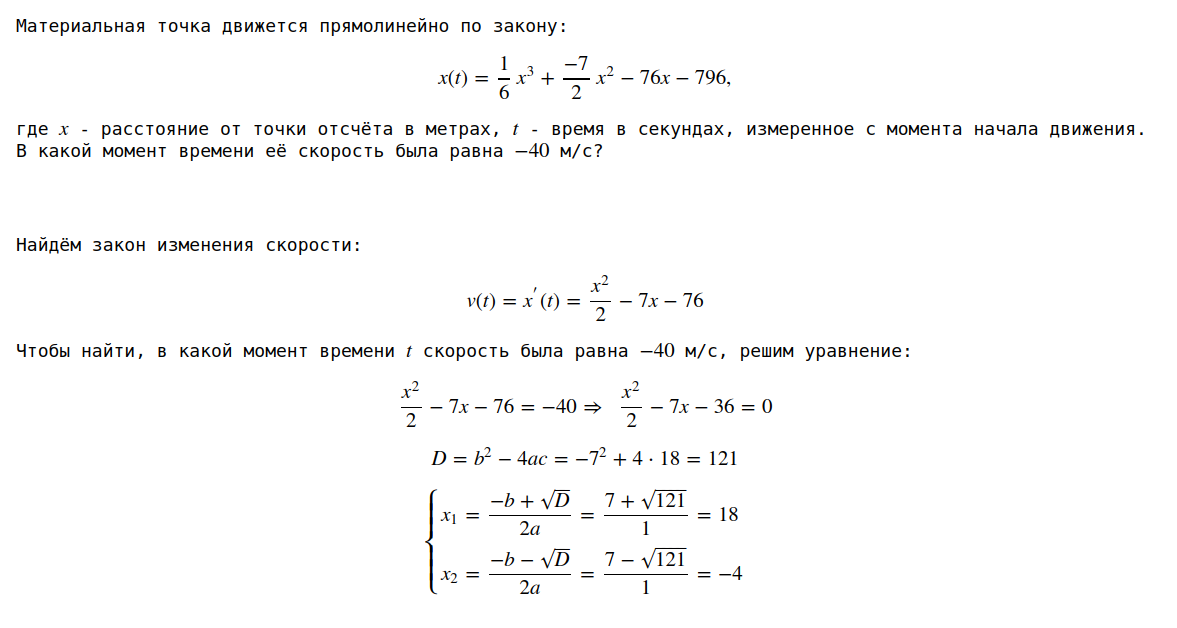
\includegraphics[width=0.85\linewidth]{VM/vch1.png}
		 		\end{figure}
		 	\begin{figure}[h]
		\centering
		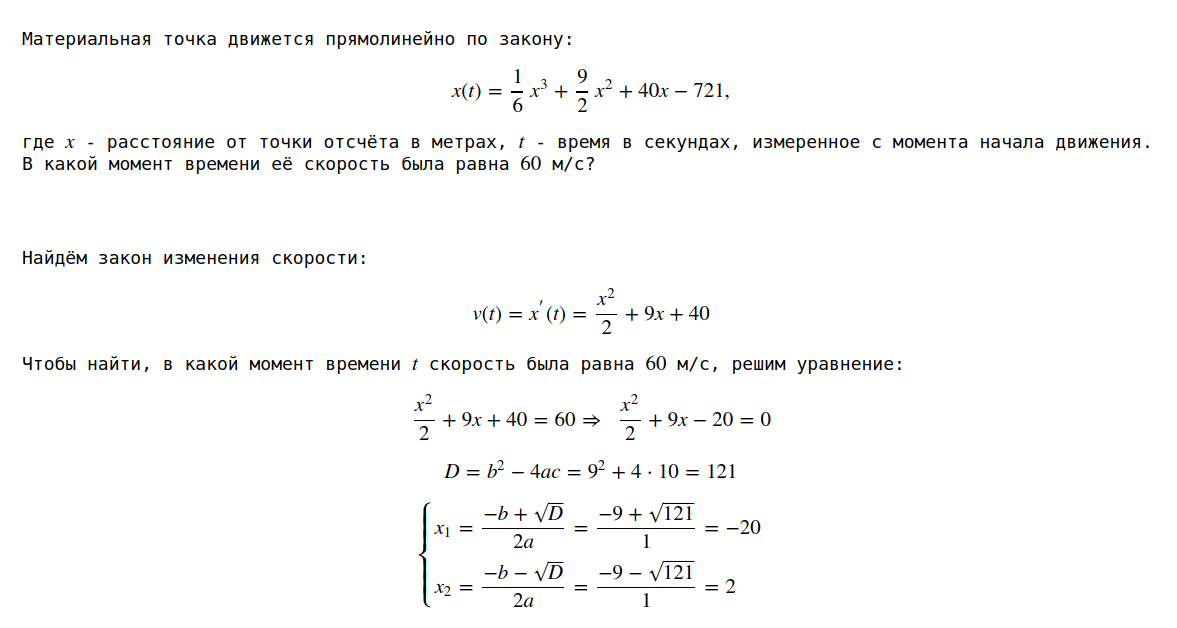
\includegraphics[width=0.85\linewidth]{VM/vch2.png}
	\end{figure}

\textbf{Задачи из ЕГЭ по математике базового уровня тип №16}

	\begin{figure}[h]
		\centering
		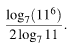
\includegraphics[width=0.11\linewidth]{VM/t16.2.png}
		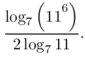
\includegraphics[width=0.11\linewidth]{VM/t16.4.png}
		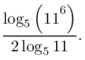
\includegraphics[width=0.11\linewidth]{VM/t16.5.png}
		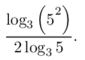
\includegraphics[width=0.11\linewidth]{VM/t16.6.png}
		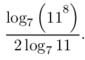
\includegraphics[width=0.11\linewidth]{VM/t16.7.png}
		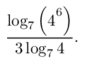
\includegraphics[width=0.11\linewidth]{VM/t16.8.png}
\end{figure}
	
\textbf{Шаблон задач}

\lstinputlisting{paragrafs/Zadachi/3}
	
Отличительной особенностью этих шаблонов от предыдущего, является другая библиотека - \texttt{setEvaluationTask}. Помимо самой генерации задачи, на основе переменных их первой части, она так же сама решает сгенерированный пример, и проверяет его ответ. 

Если ответ не является удовлетворительным, а именно таким, что пользователь просто не сможет ввести его на клавиатуре (Ответ представляет из себя бесконечную десятичную дробь, или просто очень длинную), то программа, отслеживает эту ошибку с помощью цикла \texttt{retryWhileError} и предпринимает ещё попытку составить задание с цельным ответом. Количество таких попыток указано внизу кода программы. Если за установленное число попыток, программа так и не получит правильно сгенерированную задачу, то она выведет сообщение об ошибке.

За отображение логарифма на экране здесь отвечает специальная встроенная функция: \texttt{varlog}

\textbf{Сгенерированные по шаблону задачи}

\begin{figure}[h]
		\centering
		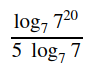
\includegraphics[width=0.11\linewidth]{VM/varlog1.png}
		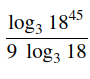
\includegraphics[width=0.11\linewidth]{VM/varlog2.png}
		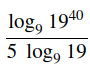
\includegraphics[width=0.11\linewidth]{VM/varlog3.png}
		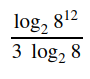
\includegraphics[width=0.11\linewidth]{VM/varlog4.png}
		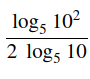
\includegraphics[width=0.11\linewidth]{VM/varlog5.png}
		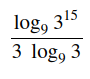
\includegraphics[width=0.11\linewidth]{VM/varlog6.png}
\end{figure}

Также эта библиотека способна сама убирать некоторые скобки, если они не влияют на решение задания, или сама выполнть арифметическую операцию. Но в некотрых случаях, это не является необходимостью. Например как в этой задаче базового типа. Здесь скобки нужны лишь для наглядности, и не оказывают никакого влияния на решение этого примера, но их всё же необходимо сохранить.

\begin{figure}[h]
		\centering
		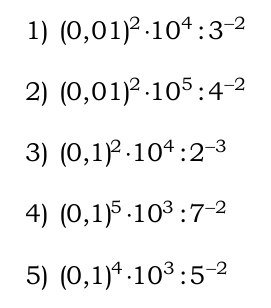
\includegraphics[width=0.4\linewidth]{VM/t16.1.png}
		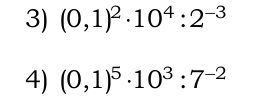
\includegraphics[width=0.4\linewidth]{VM/22.png}
\end{figure}

 Чтобы программа не высчитывала сама то, что стоит оставить, используются следующие команды:
\\ \texttt{forceBrackets} - для сохранение скобок.
\\ \texttt{divideColon} - для вывода знака деления «:».

Шаблон задачи, использующий эти специальные команды

\lstinputlisting{paragrafs/Zadachi/4}

\textbf{Сгенерированные по шаблону задания}

		\begin{figure}[h]
		\centering
		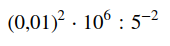
\includegraphics[width=0.35\linewidth]{VM/dv1.png}
		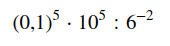
\includegraphics[width=0.35\linewidth]{VM/dv2.png}
		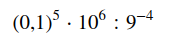
\includegraphics[width=0.35\linewidth]{VM/dv3.png}
		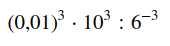
\includegraphics[width=0.35\linewidth]{VM/dv4.png}
\end{figure}

\textbf{Задача №77381 тип №6}

\begin{figure}[h]
	\centering
	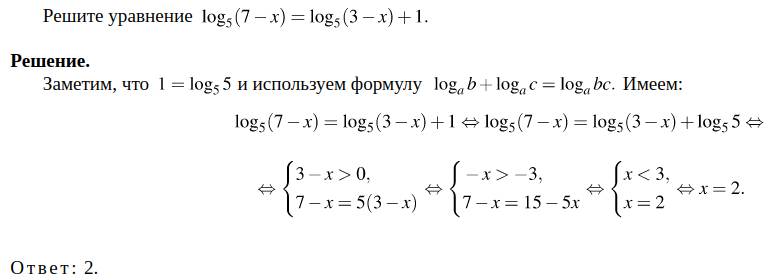
\includegraphics[width=1\linewidth]{VM/god.png}
\end{figure}

Первая часть шаблона задачи №77381
 
Здесь, помимо ввода переменных, и подбора подходящего корня, происходит проверка корня на его вхождение в ОДЗ, а также проверяется сколько знаков после запятой он имеет. В данном случае, программа контролирует, чтобы ответ имел не более 3 знаков. Сделано это, чтобы пользователю было удобнее вводить ответ.

\lstinputlisting{paragrafs/Zadachi/5}

Вторая часть шаблона задачи №77381

Ещё одной отличительной особенностью этого шаблона, является его библиотека \texttt{setAdditiveEquationTask}. Благодаря ней, части уравнения, записанные в квадратные скобки после слова \texttt{parts:} будут каждый раз переставлятся при запуске программы, что создаёт больше разнообразия в задачах, использующих этот код.

Эта часть также содержит некоторые специальные встроенный функции:
\\ \texttt{[a,b,c].slag()} – функция выводящая пример, в котором все элементы массива слагаемыми в различном порядке.
\\ \texttt{a.pow(b)} – функция возводящая число в степень
И некоторые команды из LaTeX, например: 
\\  \texttt{\textbackslash \textbackslash cdot} - выводящая знак умножения в виде точки.

\lstinputlisting{paragrafs/Zadachi/6}

\newpage

\textbf{Задачи сгенерированные по шаблону}

\begin{figure}[h]
	\centering
	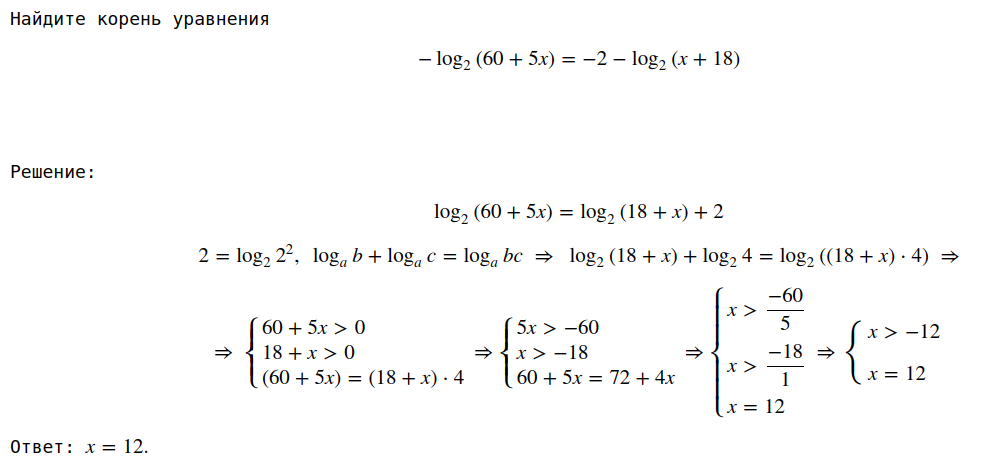
\includegraphics[width=1\linewidth]{VM/asd1.png}
	\end{figure}
	\begin{figure}[h]
	\centering
	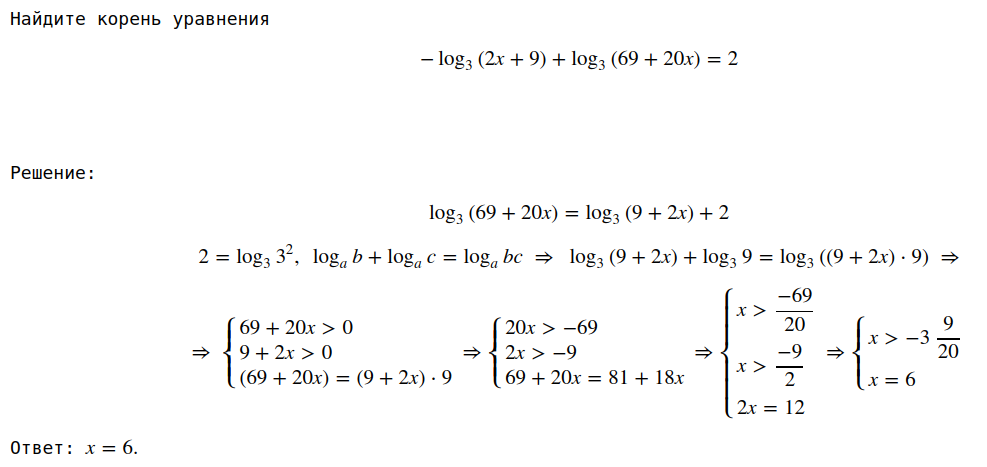
\includegraphics[width=1\linewidth]{VM/asd2.png}
\end{figure}


\textbf{Код класса арифметической прогрессии}

\lstinputlisting{paragrafs/Zadachi/7}

В классе присутсвуют функции, которые высчитывают с помощью формул определённый член прогресси, а также сумму прогрессии. 

Во второй части кода пользователь вводит значения, которые передаются в класс и принимаются в качестве аргументов функциями, после чего ответ выводится на экран.

Задачи на арифметическую прогрессию

\begin{figure}[h]
	\centering
	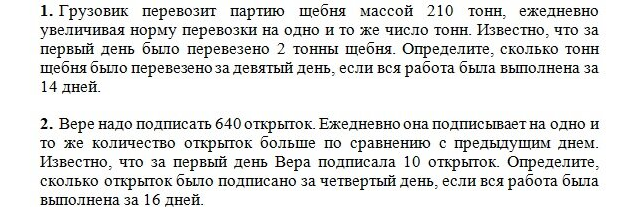
\includegraphics[width=1\linewidth]{VM/ar1.png}
	\end{figure}
	
Шаблон использующий библиотеку со встроенным классом арифметической прогрессии

\lstinputlisting{paragrafs/Zadachi/10}

\textbf{Задачи, сгенерированные по шаблонам, использующим код арифметической прогрессии.}
	\begin{figure}[h]
		\centering
		
\includegraphics[width=1\linewidth]{VM/1 (1).png}
		
\includegraphics[width=1\linewidth]{VM/2 (1).png}
		
\includegraphics[width=1\linewidth]{VM/3 (1).png}
	\end{figure}


Задачи на геометрическую прогрессию

\begin{figure}[h]
	\centering
	
\includegraphics[width=1\linewidth]{VM/ar2.png}
	
\includegraphics[width=1\linewidth]{VM/ar3.png}
	\end{figure}

\textbf{Код геометрической прогрессии}

\lstinputlisting{paragrafs/Zadachi/8}

Помимо функций, что присутсвуют и в классе арифметической прогрессии, здесь пристутсвует функция вычисляющая сумму бусконечно убывающей прогрессии. Для этого она проверяет, является ли знаменатель меньше единицы, и не является ли он меньше нуля, ведь тогда прогрессия будет знакочередующейся, и её сумму уже нельзя будет найти.

\textbf{Задачи, сгенерированные по шаблонам, использующим код 
\\геометрической прогрессии.}

	\begin{figure}[h]
		\centering
		
\includegraphics[width=1\linewidth]{VM/4 (1).png}
		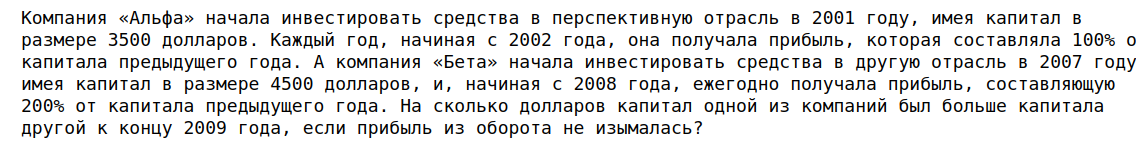
\includegraphics[width=1\linewidth]{VM/5 (1).png}
	\end{figure}
	
\textbf{Задача №26695}

	\begin{figure}[h]
		\centering
		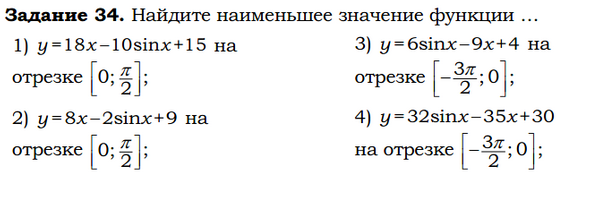
\includegraphics[width=0.95\linewidth]{VM/666.png}
	\end{figure}

\textbf{Код задачи №26695}

\lstinputlisting{paragrafs/Zadachi/8}

Одной из особенностей этого шаблона является, использующаяся в нём библиотека \texttt{setMinimaxFunctionTask}, которая берёт на себя большую часть работы по подбору значейний, а также отображению задачи на экране. Но всё же трудности могут возникнуть при подборе значений для  \texttt{primaryStep:} и \texttt{secondaryStep:}, отвещающих за первичный и вторичный перебор значений максимума или минимума соответственно. Сначала поиск проходит первичным шагом, затем в окрестности предполагаемого ответа, происходит поиск вторичным шагом. Чем меньше задать шаги поиска, тем больше будет нагрузка и дольше программа будет подбирать значение, а если сделать наоборот, и задать шаги большего размера, то увеличится скорость поиска, но пострадает точность решения.


\textbf{Задача №26695 сгенерированная по шаблону.}
	\begin{figure}[h]
		\centering
		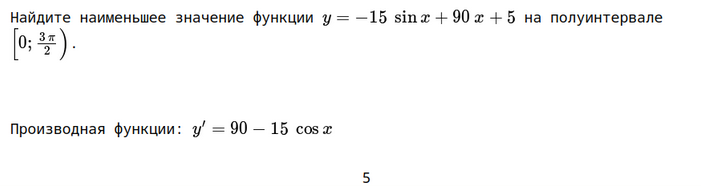
\includegraphics[width=1\linewidth]{VM/p1.png}
		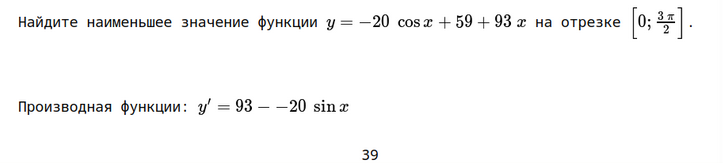
\includegraphics[width=1\linewidth]{VM/p2.png}
	\end{figure}

\textbf{Тригонометрическая задача №77492}

	\begin{figure}[h]
		\centering
		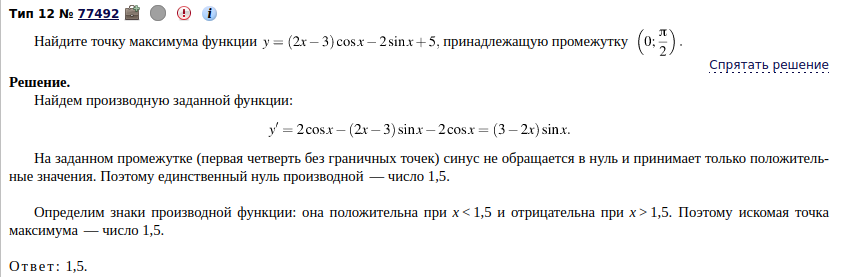
\includegraphics[width=1\linewidth]{VM/ttt.png}
	\end{figure}


\textbf{Код для задачи №77492}


\lstinputlisting{paragrafs/Zadachi/9}

В коде этой задачи не использовалась библиотека из прошлой, потому что здесь стояла другая цель. Здесь нужно найти точку максимума (минимума) функции, а не её максимальное (минимальное) значение. Также здесь, присутсвуют подробное поясненяющее решение.

\textbf{Решение тригонометрической задачи сгенерированное шаблоном}

	\begin{figure}[h]
		\centering
		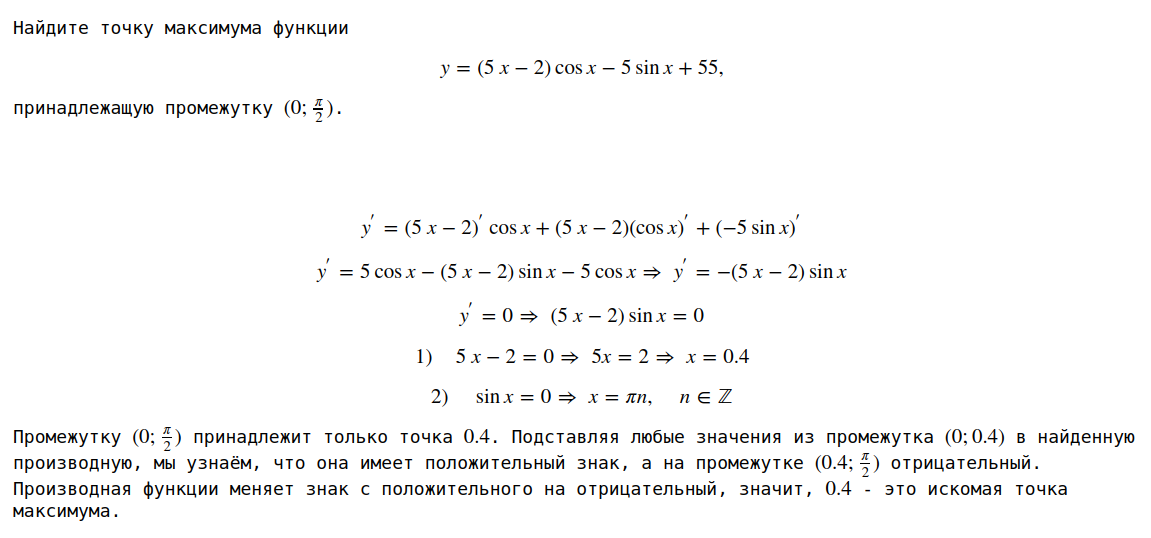
\includegraphics[width=1\linewidth]{VM/7 (1).png}
	\end{figure}
	
\newpage